\chapter{研究準備}
章の表題は,自分の論文に合わせて変更してください.
ここでは,自分が提案する手法がどのような他の理論や技術によって成り立って
いるのかを第4章で説明するための準備として,理論の説明などを行います.
\section{本章にて記すべき内容}
\begin{itemize}
\item {\bf 研究で使う理論や手法などについての説明}\\
論文や報告書を書くときに大切なことは,その論文を読者が頭から読んでいった
      ときに,最後までわからない言葉などがないように気をつけることです.
      そのために,専門用語などを使うときは必ず前もって説明をする必要があ
      ります.用語や手法(例えば,「オントロジー」,「tf・idf」など)は
知らない人はまったくわからないことなので,その説明を明確に記す必要があり
      ます.
\item {\bf 研究の背景について説明による第3章でなされる自分の研究の内容の説明への導入}\\
自分がおこなう研究の分野において,現在までにどのような研究がなされてきたのかを
説明し,自分の研究内容がそれらとどう異なり新規性があるのかを述べる.\\
\end{itemize}

\subsection{図の挿入方法}
以下に図をfigure環境をもちいて貼りつけた例をしめす.labelは文章中にその図を参照
するときのキーワードとして用いられる.figure環境を使うことにより,図目次のところに
自動的にその図とタイトルがリストアップされる.ひとつ注意することは,figure環境を使う
と\LaTeX が勝手に図の配置をおこなってしまう.これは,\LaTeX のなかで最適な場所を
選んでおこなっているのだが,われわれにとって不都合な場合も多々ある.その場合には,
文章の長さや図の大きさなどを調整して,自分たちが図を挿入したい場所に図が入るように
工夫するしかない.(この場合,図が次のページに飛んでしまっている.)

\begin{center}
\begin{figure}[htbp]
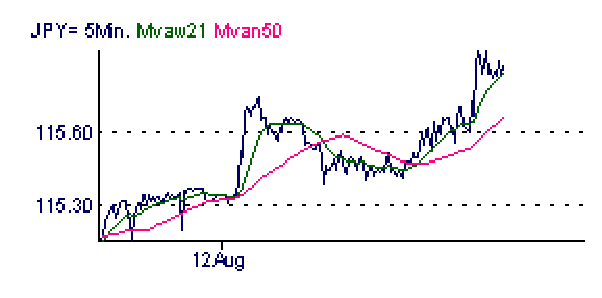
\includegraphics[totalheight=5cm]{sample1}
\caption{8月12日の円対ドルの推移}
\label{fig:exchange0812}
\end{figure}
\end{center}

また,figure環境をつかって,labelを設定したなら,あとで新たに図を挿入しても
図の番号が自動的に変更される.本文中の参照のしかたは次の括弧内の図2.1のソースを
参照のこと.(図\ref{fig:exchange0812})